% !TEX root =  ../master.tex
\chapter{Konzeption}
\section{Frontendarchitektur}
\section{Datenmodell und Datenhaltung}

Die Anwendung folgt dem \ac{MVC}-Pattern. Das heißt, die Anwendung ist aufgeteilt in 3 Bereiche:
\begin{itemize}%TODO: Hier kann man noch mehr schreiben
    \item Model\\
        Das Modell stellt den aktuellen Status bzw. den aktuellen Zustand der Anwendung dar.
    \item View\\
        Die Präsentation ist zuständig für die Darstellung der Daten und ermöglicht dem Benutzer die Interaktion mit diesen sowie die Steuerung der Anwendung.
    \item Controller\\
        Der Controller kümmert sich um die Steuerung der Anwendung. Er verwaltet die Präsentation und steuert den Datenfluss zwischen der Präsentation und dem Modell.
\end{itemize}
% \begin{wrapfigure}{r}{5.5cm}
%     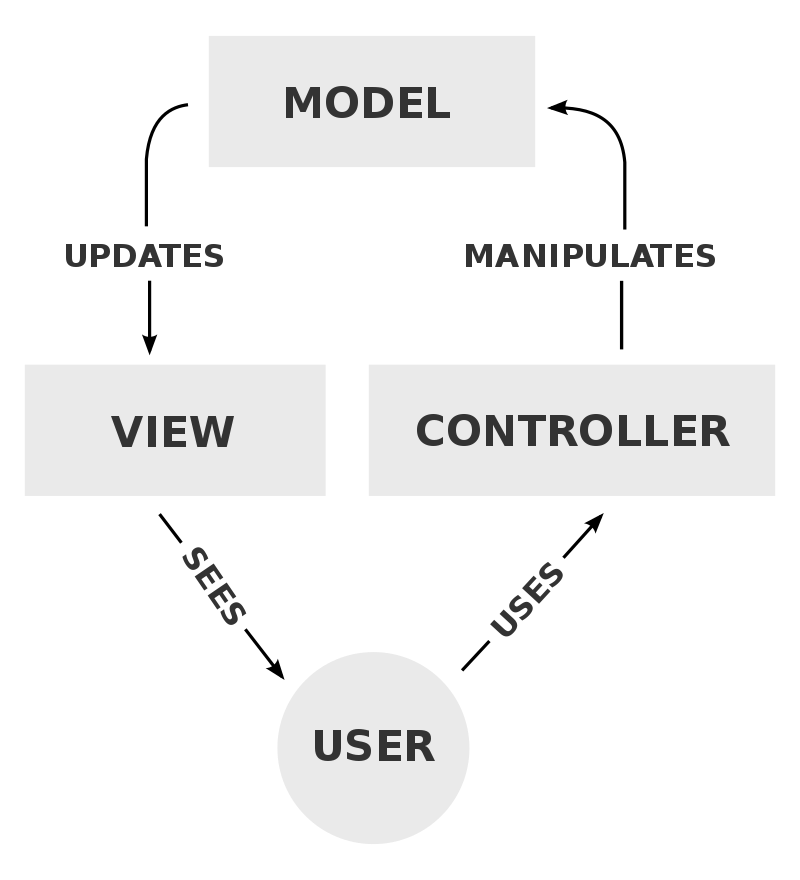
\includegraphics[width=.25\textwidth]{img/1024px-ModelViewControllerDiagram2.svg.png}
%     \caption{}
%     %TODO: https://en.wikipedia.org/wiki/Model%E2%80%93view%E2%80%93controller#/media/File:MVC-Process.svg
%   \end{wrapfigure} 

% TODO ER-Modell

Die Datenhaltung ist wie bereits beschrieben im Modell als Zustand definiert. Für die Verwaltung der Daten wird \href{https://vuex.vuejs.org/}{VueX} verwendet.
Das Modell wird hierbei als \enquote{Store} repräsentiert.
Der gesamte Store ist dabei gekapselt und definiert Funktionen zur Manipulation des internen Zustandes. Der Aufbau des Stores ist dabei konstant und ändert sich nicht abhängig der gespeicherten Daten.
Der Store besteht dabei aus:
\begin{itemize}
    \item State\\
        Der State definiert alle gespeicherten Daten. Die Anwendung überwacht den State und aktualisiert die Präsentation sobald sich eine Änderung am State ergibt.
    \item Getters\\
        Getters sind Funktionen, die dynamisch Daten aus dem State errechnen.
    \item Mutations\\
        Mutations sind Funktionen, die den State manipulieren.
        Durch die atomare, synchrone Weiße dieser Funktionen wird sichergestellt, dass nicht mehrere Änderungen gleichzeitig vorgenommen werden und der Zustand stets konsistent ist.
    \item Actions\\
        Actions sind Funktionen, die asynchrone Aktionen ausführen können. Ein Beispiel hierfür ist das Laden von Daten aus der Datenbank. Da Änderungen am State nur über Mutations ausgeführt werden können, müssen Actions am Ende ihrer Ausführung die notwendige Mutation ausführen.
\end{itemize}

Die Ausführung der Funktionen geschieht durch ein Eventsystem. Der Controller muss so nur die notwendige Event mit Eventdaten zur Bearbeitung des Zustandes erzeugen und überlässt die Ausführung dem Store. Da die Anwendung den State überwacht und die Repräsentation bzw. die UI anpasst wird die Art und Weiße, wie Daten gespeichert sind entkoppelt vom Zugriff auf diese, sowie deren Darstellung.


\subsection{Studierende}
\subsection{Dozierende}
\subsection{Kurs erstellen}
\subsection{Karteikarten-Lernsystem}
\subsection{ToDo-Liste}
\section{Datensicherheit}
\section{Datenschutz}
\section{Grundlage für Datenauswertung}
% Hier Verweise auf Aubau und Bezug zum leichten Ausbau, etc.